\documentclass{article}
\usepackage{graphicx}
\usepackage{lmodern} % Fix the font size warnings
\usepackage{fancyhdr} % Required for custom headers
\usepackage{lastpage} % Required to determine the last page for the footer
\usepackage{extramarks} % Required for headers and footers
\usepackage{graphicx} % Required to insert images
\usepackage{xfrac} % Nice fractions
\usepackage{amsmath}

\usepackage{multicol}

% Margins
\topmargin=-0.5in
\evensidemargin=0in
\oddsidemargin=-0.5in
\textwidth=7.5in
\textheight=9.0in
\headsep=0.25in 

% paragraphs
\usepackage{parskip}

\pagestyle{fancy}

\rhead{Main courses}
\lhead{\textbf{Caitlyn's Fried Chicken Fingers}}
\chead{}
\title{Caitlyn's Fried Chicken Fingers}

\begin{document}
Sometimes you just need to start with someone's recipe and then tweak the hell out of it until it works.
This is one of those times. This started as a TikTok recipe, but, well, it was a little rough. Not all
the ingredients were listed. Actually, let's face it, \emph{nothing} was really written down. There were
two places where "1 Tbsp All-purpose" was listed. "All-purpose \emph{what}", exactly? Anyway, Caitlyn wanted to make these and took a real run at them. After the first three pieces came out
less than perfect (in Caitlyn's words), she made some changes, and this is the result.

\begin{multicols}{2}

    \textbf{Ingredients for the dry part}

    \begin{itemize}
        \setlength\itemsep{-0.5em}
        \item 4 cups flour
        \item 2 tablespoons baking powder
        \item 2 tablespoons garlic powder
        \item 2 tablespoons onion powder
        \item 1 tablespoon cayenne pepper
        \item 1 teaspoon black pepper
        \item 1 teaspoon salt

        \item cayenne, chili powder, ancho chili, or other flavorful spice for sprinkling, to taste
    \end{itemize}

    \columnbreak

    \textbf{Ingredients for the wet part}

    \begin{itemize}
        \setlength\itemsep{-0.5em}
        \item 1\sfrac{1}{4} cup cultured buttermilk
        \item \sfrac{1}{4} cup pickle juice
        \item 1 tablespoon miced garlic
        \item \sfrac{1}{2} tablespoon garlic powder
        \item \sfrac{1}{2} tablespoon onion powder
        \item 1 tablespoon cayenne pepper
        \item 1 tablespoon black pepper
        \item 1 tablespoon baking soda

        \item 1\sfrac{1}{2} pounds (one package) chicken tenders
    \end{itemize}

\end{multicols}

\textbf{Directions}

Cut chicken into smallish pieces (about 2 ounces each) and pound flat in a double zipper lock bag. You can
use your hands or a mallet. Just don't make them too thin. Nobody likes a thin chicken finger. Set this aside.

Combine all the dry ingredients in a medium-sized bowl. Combine all the wet ingredients in a medium-sized bowl. In a few minutes this should start to bubble on its own. This
is a good thing because it makes the batter nice and light.

Bring a heavy bottom dutch oven with about 2 inches of canola, corn, or other vegetable oil to somewhere between
365 and 375 degrees. It's important that the oil remain in this range. Too hot and you'll burn the outside of the
chicken, but leave the inside raw. Too low and it'll take forever to cook while soaking up all the oil. Neither
are a win. Later, when frying the chicken, keep an eye on this temperature and adjust as necessary.

When the oil is ready drop a few pieces of the chicken into the buttermilk batter and make sure they get fully
covered. Pick them up one at a time and let the buttermilk drip off a bit. Dip each piece of battered chicken into
the dry ingredients and make sure it gets flour all the way around. Place the battered chicken on a tray.

When you have 4 or 5 pieces ready it's time to drop them into the hot oil. Shake off any excess flour before putting
the tenders in the oil. Cook about 4 minutes on one side, turn over with a long-handled tong, then cook until they are
at least 165 degrees inside. Place them on a paper towel and sprinkle with the cayenne and chili powder. The more, the
spicier. And spicier is good.

\begin{figure}
    \centering
    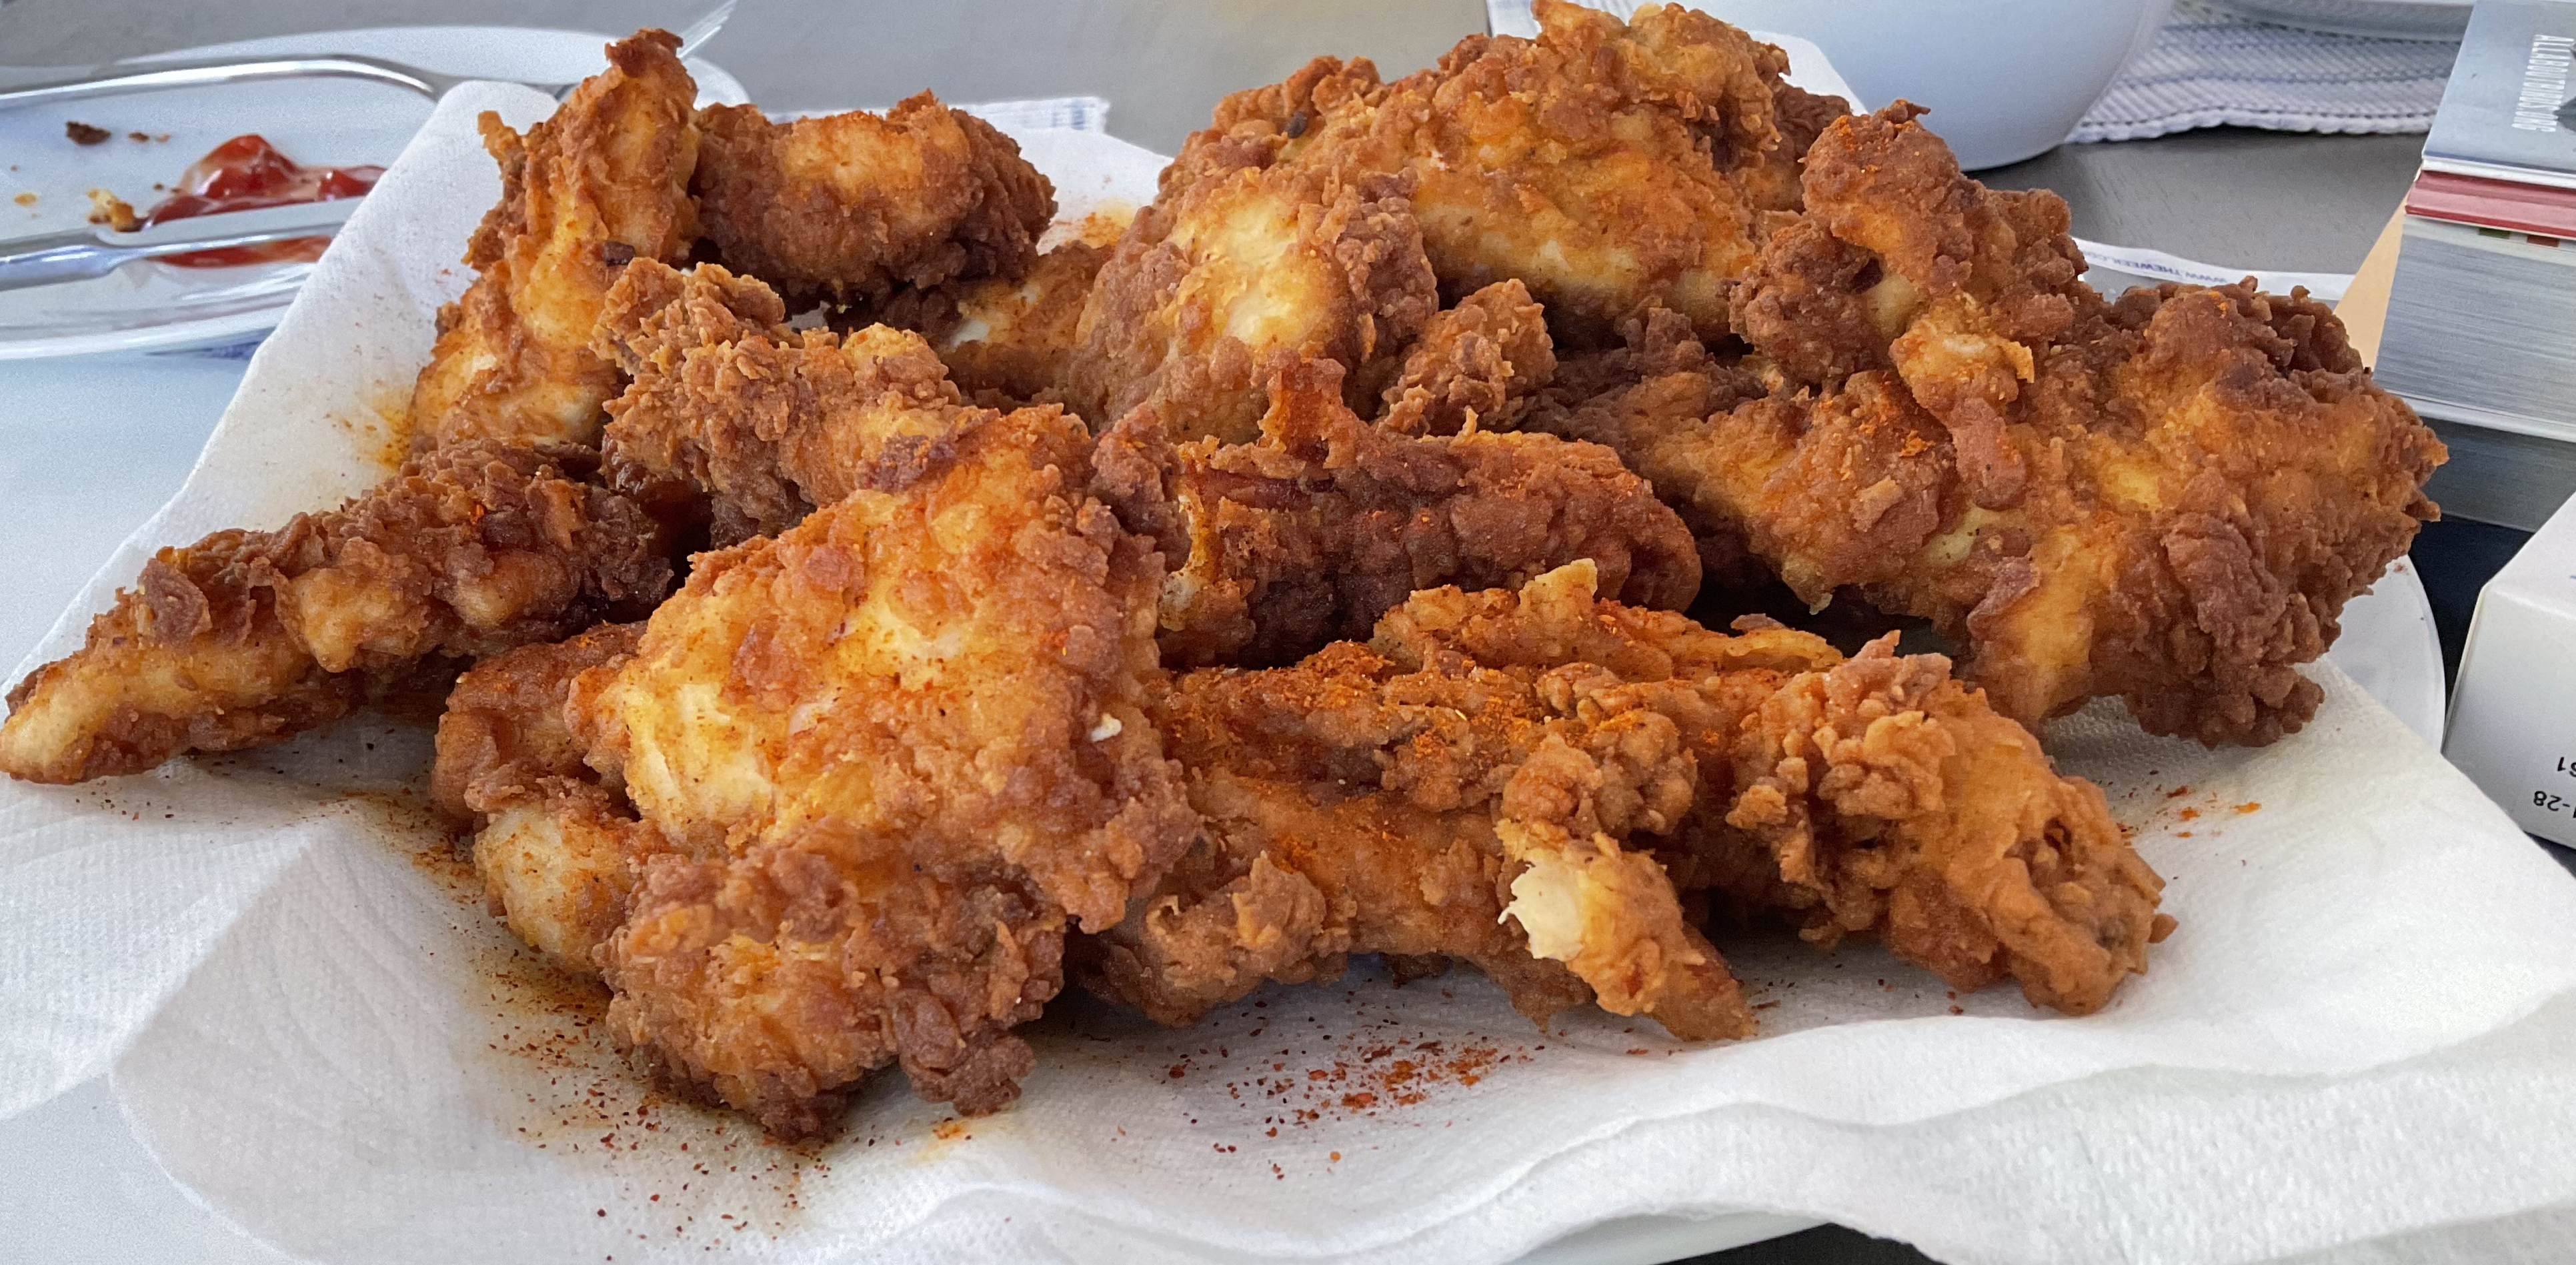
\includegraphics[scale=0.095]{fried-chicken.png}
\end{figure}

\end{document}
